\documentclass[12pt, a4paper, english]{report}

\usepackage{babel}
\usepackage[T1]{fontenc}
\usepackage[utf8]{inputenc}

\usepackage{float}
\usepackage{enumerate}
\usepackage{enumitem}
\usepackage{multicol}
\usepackage{multirow}
\usepackage{cite}
\usepackage{appendix}
\usepackage{tabularx}

\usepackage{ragged2e}

\usepackage{rotating}
\usepackage[bookmarks,pdfencoding=unicode,colorlinks=true,citecolor=blue,linkcolor=black,urlcolor=blue]{hyperref}
\usepackage[normalem]{ulem}			% package for strikethrough
\newcommand{\strike}[1]{\sout{#1}}	% strikethrough
\usepackage{lipsum}
\graphicspath{{img/}}

% Basic formatting
\setlength{\parindent}{0em}
\newcommand{\ppar}{\par\medskip}

\usepackage{color}

\definecolor{mygreen}{rgb}{0,0.6,0}
\definecolor{mygray}{rgb}{0.5,0.5,0.5}
\definecolor{mymauve}{rgb}{0.58,0,0.82}

\definecolor{commentGreen}{RGB}{128,127,41}
\definecolor{stringGreen}{RGB}{0,127,38}
\definecolor{keywordRed}{RGB}{151,0,11}
\definecolor{typePurple}{RGB}{128,3,82}
\definecolor{variableBlue}{RGB}{0,0,255}
\definecolor{annotationRed}{RGB}{198,4,38}
\definecolor{annotationBlue}{RGB}{32,21,223}

% Code
\usepackage[procnames]{listings}
\lstset{ %
	aboveskip={-0.2\baselineskip},			% space before box
    backgroundcolor=\color{white},		% choose the background color
    basicstyle=\footnotesize\ttfamily,	% the size of the code
    breakatwhitespace=false,			% if automatic breaks happen at whitespace
    breaklines=true,					% sets automatic line breaking
%    captionpos=b,						% sets the caption-position to bottom
    commentstyle=\color{mygray},		% comment style
    deletekeywords={...},				% delete keywords from the given language
    escapeinside={\%*}{*)},				% if you want to add LaTeX within your code
    extendedchars=true,					% lets you use non-ASCII characters
    frame=single,						% adds a frame around the code
    keepspaces=true,					% keeps spaces in text, for indentation
    keywordstyle=\color{blue},			% keyword style
    otherkeywords={*,...},				% add more keywords to the set
    numbers=left,						% where to put the line-numbers
%    numbersep=-20pt,					% line-numbers distance from the code
    numberstyle=\tiny\color{mymauve},	% style for the line-numbers
    rulecolor=\color{black},			% the frame-color
    showspaces=false,					% show spaces everywhere adding particular underscores; it overrides 'showstringspaces'
    showstringspaces=false,				% underline spaces within strings only
    stepnumber=1,						% the step between two line-numbers
    stringstyle=\color{mygreen},		% string literal style
    tabsize=4,	% sets default tabsize
    title=\lstname,						% show the filename
%    identifierstyle=\color{orange}		% identifiers colors
}
\newcommand{\cod}[1]{\lstinline�#1�}

% from https://tex.stackexchange.com/questions/79747/advanced-use-of-listings-package
\lstdefinelanguage[drl]{Drools}{
    sensitive=true,
    keywordsprefix=\$,
    alsoletter={:, },
    morekeywords=[2]{long,int,boolean,double,float,enum},
    morekeywords=[3]{declare,end,extends,from,insert,modify,not,new,no loop,query,retract,rule,salience,then,this,when, eval},
    morekeywords=[4]{after,before,during,over window:length,over window:time,overlaps},
    morekeywords=[5]{{no loop},over window:length,over window:time},
    morecomment=[l]{//},
    morecomment=[s]{/*}{*/},
    moredelim=[s][\color{annotationRed}\itshape]{@}{)},
    moredelim=[s][\color{annotationBlue}\itshape]{@[}{]},
    morestring=[b]",
    morestring=[d]',
%%% default style
    basicstyle=\normalfont\ttfamily,
    % identifierstyle=\normalfont,
    commentstyle=\color{commentGreen}\itshape,
    keywordstyle=\color{keywordRed}\bfseries,
    keywordstyle=[1]\color{variableBlue}\itshape,
    keywordstyle=[2]\color{typePurple}\bfseries,
    keywordstyle=[3]\color{keywordRed}\bfseries,
    keywordstyle=[4]\color{keywordRed}\bfseries,
    keywordstyle=[5]\color{stringGreen}\bfseries,
    stringstyle=\color{stringGreen}
}[comments,keywords,strings]

\def\bullet{\(\triangleright\)}
%\renewcommand{\familydefault}{\sfdefault}
%\renewcommand{\thesection}{\arabic{section}} % section numbers like [1..]

\begin{document}

\begin{titlepage}
\begin{center}
~\\[2cm]

\includegraphics[width=0.5\textwidth]{logo}\\[3.5cm]
\hrule height 1pt
\vspace{5mm}
{\Huge University timetable scheduling}
\vspace{3mm}
\hrule height 1pt
\vspace{1cm}
{\Large Bachelor Project Report}\\[3mm]
{\Large Aron Fiechter}\\[3mm]
{\Large 2018}\\[3.5cm]
{\large Advisor: Prof. Dr. Michele Lanza}\\[3mm]
{\large Assistants: Dr. Andrea Mocci, Dr. Luca Ponzanelli}
\end{center}
\end{titlepage}

\tableofcontents
\newpage

%%%%%%%%%%%%%%%%%%%%%%%%%%%%%%%%%%%%%%%%%%%%%%%%%%%%%%%%%%%%%%%%%%%%%%%%%%%%%%%%
%%%%%%%%%%%%%%%%%%%%%%%%%%%%%%%%%%%%%%%%%%%%%%%%%%%%%%%%%%%%%%%%%%%%%%%%%%%%%%%%
\chapter*{Abstract}
Creating and managing timetables of courses is an issue for many institutions because of the various constraints that need to be respected in the planning.
This is an even harder problem if the data needed to describe the planning problem and its constraints is not well curated and stored in several different places, a situation that often leads to a long and tedious manual work in creating the timetables.
In this project, we automate the process by means of state of the art tools to solve planning problems.
We describe the design and implementation of a web application that offers an automated timetable creator wrapped in a user friendly web interface.

\newpage

%%%%%%%%%%%%%%%%%%%%%%%%%%%%%%%%%%%%%%%%%%%%%%%%%%%%%%%%%%%%%%%%%%%%%%%%%%%%%%%%
%%%%%%%%%%%%%%%%%%%%%%%%%%%%%%%%%%%%%%%%%%%%%%%%%%%%%%%%%%%%%%%%%%%%%%%%%%%%%%%%
\chapter{Introduction}
%_______________________________________________________________________________
\section{Motivation}
Creating a school timetable is a difficult problem because of the various constraints that need to be respected, such as different room sizes, instructor availability, elective courses, and different frequency of courses.\par
Moreover, a timetable created for a specific academic year might be partially or totally unusable the next year, because of changes in the program (e.g. a course is cancelled or moved to a different semester) or in the constraints data. This fact requires many institutions to recreate a new timetable from scratch every year.\par
This task is even harder if the data for the courses, rooms and all the constraints is not curated and it is stored in separate and unrelated locations. Even worse, some constraints (such as instructor availability) might arise during planning, making the whole process even more tedious, requiring further (manual) work.\par
Once a viable schedule is created, it is often necessary to change some details, for example by moving some lectures to different periods or different rooms. This could however violate constraints, and checking this manually, while not very hard, still takes some time, and might require moving other lectures to accommodate the initial change.

%_______________________________________________________________________________
\section{Problem}
School timetabling is an NP hard planning problem\cite{CLRS}. The problem consists in scheduling a set of lectures on a weekly timetable. A single lecture can vary on two variables, which are period (identifying a specific slot during the week) and room.\par
The search space is huge; we can calculate it using a simple formula\footnote{\url{http://docs.optaplanner.org/latest/optaplanner-docs/html\_single/index.html\#searchSpaceSize}}:
\[
	(p \times r)^l
\]
where \(p\) is the number of possible periods on the weekly timetable, \(r\) is the number of available rooms and \(l\) is the number of lectures that need to be scheduled.\par
For example, take the spring semester of the Bachelor of Informatics at USI Lugano, which (at the time of writing) entails 14 courses, each with a specific number of lectures (calculated with respect to the ECTS weight). The total number of lectures of all courses is 70; the Faculty of Informatics has 7 rooms available, and a school week is of 40 periods (5 days, each with 8 time slots). We have:
\[
	(p \times r)^l = (40\cdot7)^{70} = 280^{70} \approx 2\cdot10^{171}
\]
Even with constraints in place, the search space remains very large. The search space contains all possible solutions, including the optimal solution, which is not necessarily feasible\footnote{according to the definitions in the OptaPlanner documentation available at \url{http://docs.optaplanner.org/latest/optaplanner-docs/html\_single/index.html\#aPlanningProblemHasAHugeSearchSpace}}. There might be no feasible solutions: Consider the case of scheduling two lectures over one single possible period, in one single available room. The only solution is to schedule both lectures in the same room during that single period, which of course is not a feasible solution.

%_______________________________________________________________________________
\section{Goal}
The goal of this project is to create a web application that automates the process of creating a school timetable.\par
The web application is an interface to a constraint solver, which lives on the back end.\par
Given the problem data and a set of constraints, the solver computes a good solution and returns it as a list of lectures. The solution is proposed to the user, which can then customize it by moving lectures to preferred times or rooms and locking them in place. The customized solution can then be fed back to the solver which can refine it while keeping the locked lectures in place.

%_______________________________________________________________________________
\section{Approach}
The solver, which is the core of the application, has been developed using OptaPlanner\footnote{\url{https://www.optaplanner.org/}}, a state of the art constraint solver which provides many optimization algorithms to solve planning problems.\par
The interface to the solver, that is the back end of the application, is a server written in Scala\footnote{\url{https://www.scala-lang.org/}}, which exposes a GraphQL\footnote{\url{https://graphql.org/}} API.\par
The front-end application is implemented in {Polymer 2.x}\footnote{\url{https://www.polymer-project.org/}} and Typescript\footnote{\url{https://www.typescriptlang.org/}}, and uses FullCalendar\footnote{\url{https://fullcalendar.io/}}, a JavaScript event calendar, to visualize and manage timetables.


%%%%%%%%%%%%%%%%%%%%%%%%%%%%%%%%%%%%%%%%%%%%%%%%%%%%%%%%%%%%%%%%%%%%%%%%%%%%%%%%
%%%%%%%%%%%%%%%%%%%%%%%%%%%%%%%%%%%%%%%%%%%%%%%%%%%%%%%%%%%%%%%%%%%%%%%%%%%%%%%%
\chapter{State of the art}

This chapter gives an overview of what it means to solve a planning problem  (Section \ref{sec:planning}) and explains on a high level how the chosen solver, OptaPlanner, can be used to define such a problem and solve it (Section \ref{sec:optaplanner}).

%_______________________________________________________________________________
\section{Planning problems\label{sec:planning}}
A planning problem\footnote{\url{http://docs.optaplanner.org/latest/optaplanner-docs/html_single/index.html\#whatIsAPlanningProblem}} is an optimization problem that aims to minimize or maximize a goal using a set of resources under specified constraints. Some examples:
\begin{itemize}[label=\bullet]
\item Minimizing travel time on a cyclic path to visit a set of cities, visiting every city exactly once. This is widely known as the traveling salesman problem, for short TSP\footnote{\url{https://en.wikipedia.org/wiki/Travelling_salesman_problem}}.
\item Arranging \(n\) queens on an \(n \times n\) chessboard so that no queen can eat any other queen.
\item Assigning talks of a conference each to a time slot and a room so that several constraints are satisfied such as no overlapping, preferred rooms for some speakers, etc.
\item Assigning lectures to a room and a period in a weekly timetable. This is the problem that we aim to solve in this project.
\end{itemize}
Planning problems are in general NP-hard or NP-complete. For most of these problems, a brute force approach doesn't work except for very small instances. Therefore, it is common to use meta-heuristic algorithms to find an approximate solution which is good enough. Finding the best solution is usually not worth the computational effort needed, and approximate solutions are used instead.

%_______________________________________________________________________________
\section{OptaPlanner\label{sec:optaplanner}}
OptaPlanner is a constraint solver which can solve planning problems (such as the ones described in Section \ref{sec:planning}) given a description of the solution of the problem together with a mechanism to compute its score. The solution contains a list of planning entities (in our case the lectures) with customizable variables. The solver optimizes the score of the solution by modifying the values of the variables. Finally, problem facts specify the constant aspects of each problem instance (e.g., courses, rooms).\par
The library provides an detailed guide on how to implement a solver. The solver can be configured to choose different construction heuristics (such as First Fit, First Fit Decreasing, Cheapest Insertion, etc.) in the first phase of solving and different algorithms for the local search phase. Local search algorithms include Simulated Annealing, Tabu Search, and can be combined for increased efficacy.\par
It is possible to add a filter class for the planning entities, which excludes some of the entities from planning (from being modified); in our case, this is perfect to exclude locked lectures during refinement.\par
Other mechanisms are available, such as classes to assign a difficulty value to planning entities (so that harder entities can be initialised first during the construction heuristic phase) or to sort planning variables by weight.\par
%For more information on OptaPlanner, see appendix \ref{appendix:optaplanner}.

%%%%%%%%%%%%%%%%%%%%%%%%%%%%%%%%%%%%%%%%%%%%%%%%%%%%%%%%%%%%%%%%%%%%%%%%%%%%%%%%
%%%%%%%%%%%%%%%%%%%%%%%%%%%%%%%%%%%%%%%%%%%%%%%%%%%%%%%%%%%%%%%%%%%%%%%%%%%%%%%%
\chapter{Approach}

This chapter illustrates the main part of the approach, that is the implementation of the application. Section \ref{sec:problem} defines the course timetabling planning problem on a conceptual level. Section \ref{sec:technologies} gives an overview of the chosen technologies, explaining the architecture and the role of each part. Section \ref{sec:domain} describes the modelling of the problem domain to be used with the constraint solver, OptaPlanner. Section \ref{sec:constraints} examines how the constraints have been included in the score calculation. Section \ref{sec:solver} provides a brief description of the wrapper of the solver on the server side. Section \ref{sec:graphql} depicts the server endpoint interface that allows the client side to interact with the solver. Finally, section \ref{sec:polymer} describes the implementation of the web application demo.

%_______________________________________________________________________________
\section{Problem definition\label{sec:problem}}
The timetable scheduling problem aims to arrange a set of lectures in a weekly schedule with the goal of minimizing conflicts. The problem is defined according to the existing definition by the {International Timetabling Competition}\footnote{\url{http://www.cs.qub.ac.uk/itc2007/curriculmcourse/course\_curriculm\_index.htm}}. Each problem instance consists of:
\begin{itemize}[label=\bullet]
\item a list of courses: Each course has a name, a list of instructors who teach the course, a list of semesters the course is taught in, the number of lectures the course entails, %TODO is "entails" the correct term?
the minimum number of days these lectures should be spread out on, and the number of students registered for the course.
\item a list of periods: Each period is defined by a day of the week (usually between Monday and Friday) and a time slot during the day (e.g. in the range 0-7, with four slots of one hour in the morning and four in the afternoon).
\item a list of unavailable periods: Each unavailable period points to a course and to a period, indicating that the course cannot have any lecture in that specific period.
\item a list of rooms: Each room has a name and a capacity.
\end{itemize}

A solution consists of a list of lectures, each with an assigned room and a period, representing a weekly occurrence of a course in the schedule. Each solution has a score, which is calculated according to set weights related to the constraints. The score is separated in two parts (or levels): a hard score and a soft score. If a solution \(A\) has a worse hard score than another solution \(B\), then \(A\) is worse than \(B\), regardless of what the soft scores are. The hard score relates to hard constraints, while the soft score relates to soft constraints.\par
Hard constraints usually model physical limitations; in our case there are five, and we list them in Table \ref{tab:hard}.
\begin{table}[h!]
\begin{tabularx}{\textwidth}{|>{\hsize=.6\hsize\linewidth=\hsize\RaggedRight}X|
>{\hsize=1.4\hsize\linewidth=\hsize}X|}\hline
Instructor conflict & An instructor must not have two lectures in the same period.\\\hline
Semester conflict   & A semester must not have two lectures in the same period.\\\hline
Course conflict     & A course cannot have two lectures in the same period.\\\hline
Room occupancy      & Two lectures must not be in the same room in the same period.\\\hline
Room capacity       & A room capacity should not be less than the number of students in the course.\\\hline
Unavailable period  & A specific lecture must not be assigned to a specific period.\\\hline
\end{tabularx}
\caption{Hard constraints \label{tab:hard}}
\end{table}

Soft constraints model limitations which do not violate physical reality but which satisfy specific preferences about how the solution should be. Our model has four soft constraint, and we list them in Table \ref{tab:soft}.
\begin{table}[h!]
\begin{tabularx}{\textwidth}{|>{\hsize=.6\hsize\linewidth=\hsize\RaggedRight}X|
>{\hsize=1.4\hsize\linewidth=\hsize}X|}\hline
Minimum working days & Lectures of the same course should be spread out into a minimum number of days\\\hline
Semester compactness & Lectures belonging to the same curriculum should be adjacent to each other (so in consecutive periods if they are on the same day)\\\hline
Room stability       & Lectures of the same course (and possibly even those of the same semester) should be assigned to the same room\\\hline
Lecture pairs        & Lectures of the same course should be scheduled in blocks of two\\\hline
%Daily workload       & Every day should have a similar number of lectures (avoid days with few and full days)\\\hline
%Course weekly span   & Courses with more than one minimum different days required should not have lectures on consecutive days\\\hline
\end{tabularx}
\caption{Soft constraints \label{tab:soft}}
\end{table}
%\newpage%TODO:REMOVE
Each constraint has an associated value which influences the score. In our case, all values are negative, so the highest score possible is \cod{0hard/0soft}. The way constraints are associated with scores can vary. For example, if the room capacity constraint is violated, each student above the capacity could count as 1 point of penalty, or we could make each student count 2, or use a standard value of 10 points of penalty, regardless of how much the room is over capacity.

%_______________________________________________________________________________
\section{Technologies\label{sec:technologies}}
The core solver implementation makes use of a state of the art library for solving planning problems called OptaPlanner.\par
The server side of the web application is implemented in Scala, a relatively young general-purpose programming language, using Akka HTTP\footnote{\url{https://doc.akka.io/docs/akka-http/current/}}. It exposes an interface to in-memory data and to the solver using GraphQL, which is a query language that allows the user to retrieve data with high precision using a single request. GraphQL is an alternative to REST that allows the client to specify the structure of the requested data, avoiding the need for further requests. The GraphQL endpoint is also implemented in Scala using Sangria GraphQL\footnote{\url{http://sangria-graphql.org/}}.\par
The client side is implemented as a Polymer 2.x application (with TypeScript instead of JavaScript), where Polymer is a library to build Web Components\footnote{\url{https://www.webcomponents.org/}}.

%_______________________________________________________________________________
\section{Domain model for OptaPlanner\label{sec:domain}}
We modelled the problem domain according to what OptaPlanner expects.\par
The implementation is done in Scala, although for some features we had to use Java syntax; it is similar to the existing Java implementation available in the \cod{curriculumcourse} program available in the OptaPlanner examples\footnote{\url{https://github.com/kiegroup/optaplanner/tree/master/optaplanner-examples}}.\par
The main solution class, called \cod{Schedule}, contains all the lists of all problem facts (\cod{Period}s, \cod{Day}s, \cod{TimeSlot}s, \cod{Semester}s, \cod{Instructor}s, \cod{Room}s, \cod{Course}s, \cod{UnavailablePeriod}s), the list of planning entities (\cod{Lecture}) and the score (\cod{HardSoftScore}).\par
The \cod{Lecture} class implements a Planning Entity, which is what the solver can mutate in order to improve solutions. The two fields that a \cod{Lecture} can mutate of are \cod{period} and \cod{room} (of type \cod{Period} and \cod{Room}, respectively).\par
However, if a the \cod{locked} field of the lecture is set to \cod{true}, the solver ignores that \cod{Lecture} and only varies the unlocked ones. The score still takes into account all lectures, regardless of their locked value. It is important to say that a \cod{Lecture} that is locked \emph{must} have a non-null value for both its \cod{room} and \cod{period}.\par
The diagram (Figure \ref{fig:domainUML}) representing the problem shows the solution class (\cod{Schedule}) in green, the planning entity (\cod{Lecture}) in red and the problem facts in blue. Only the relevant fields are shown.\par
\begin{figure}[h]
\centering
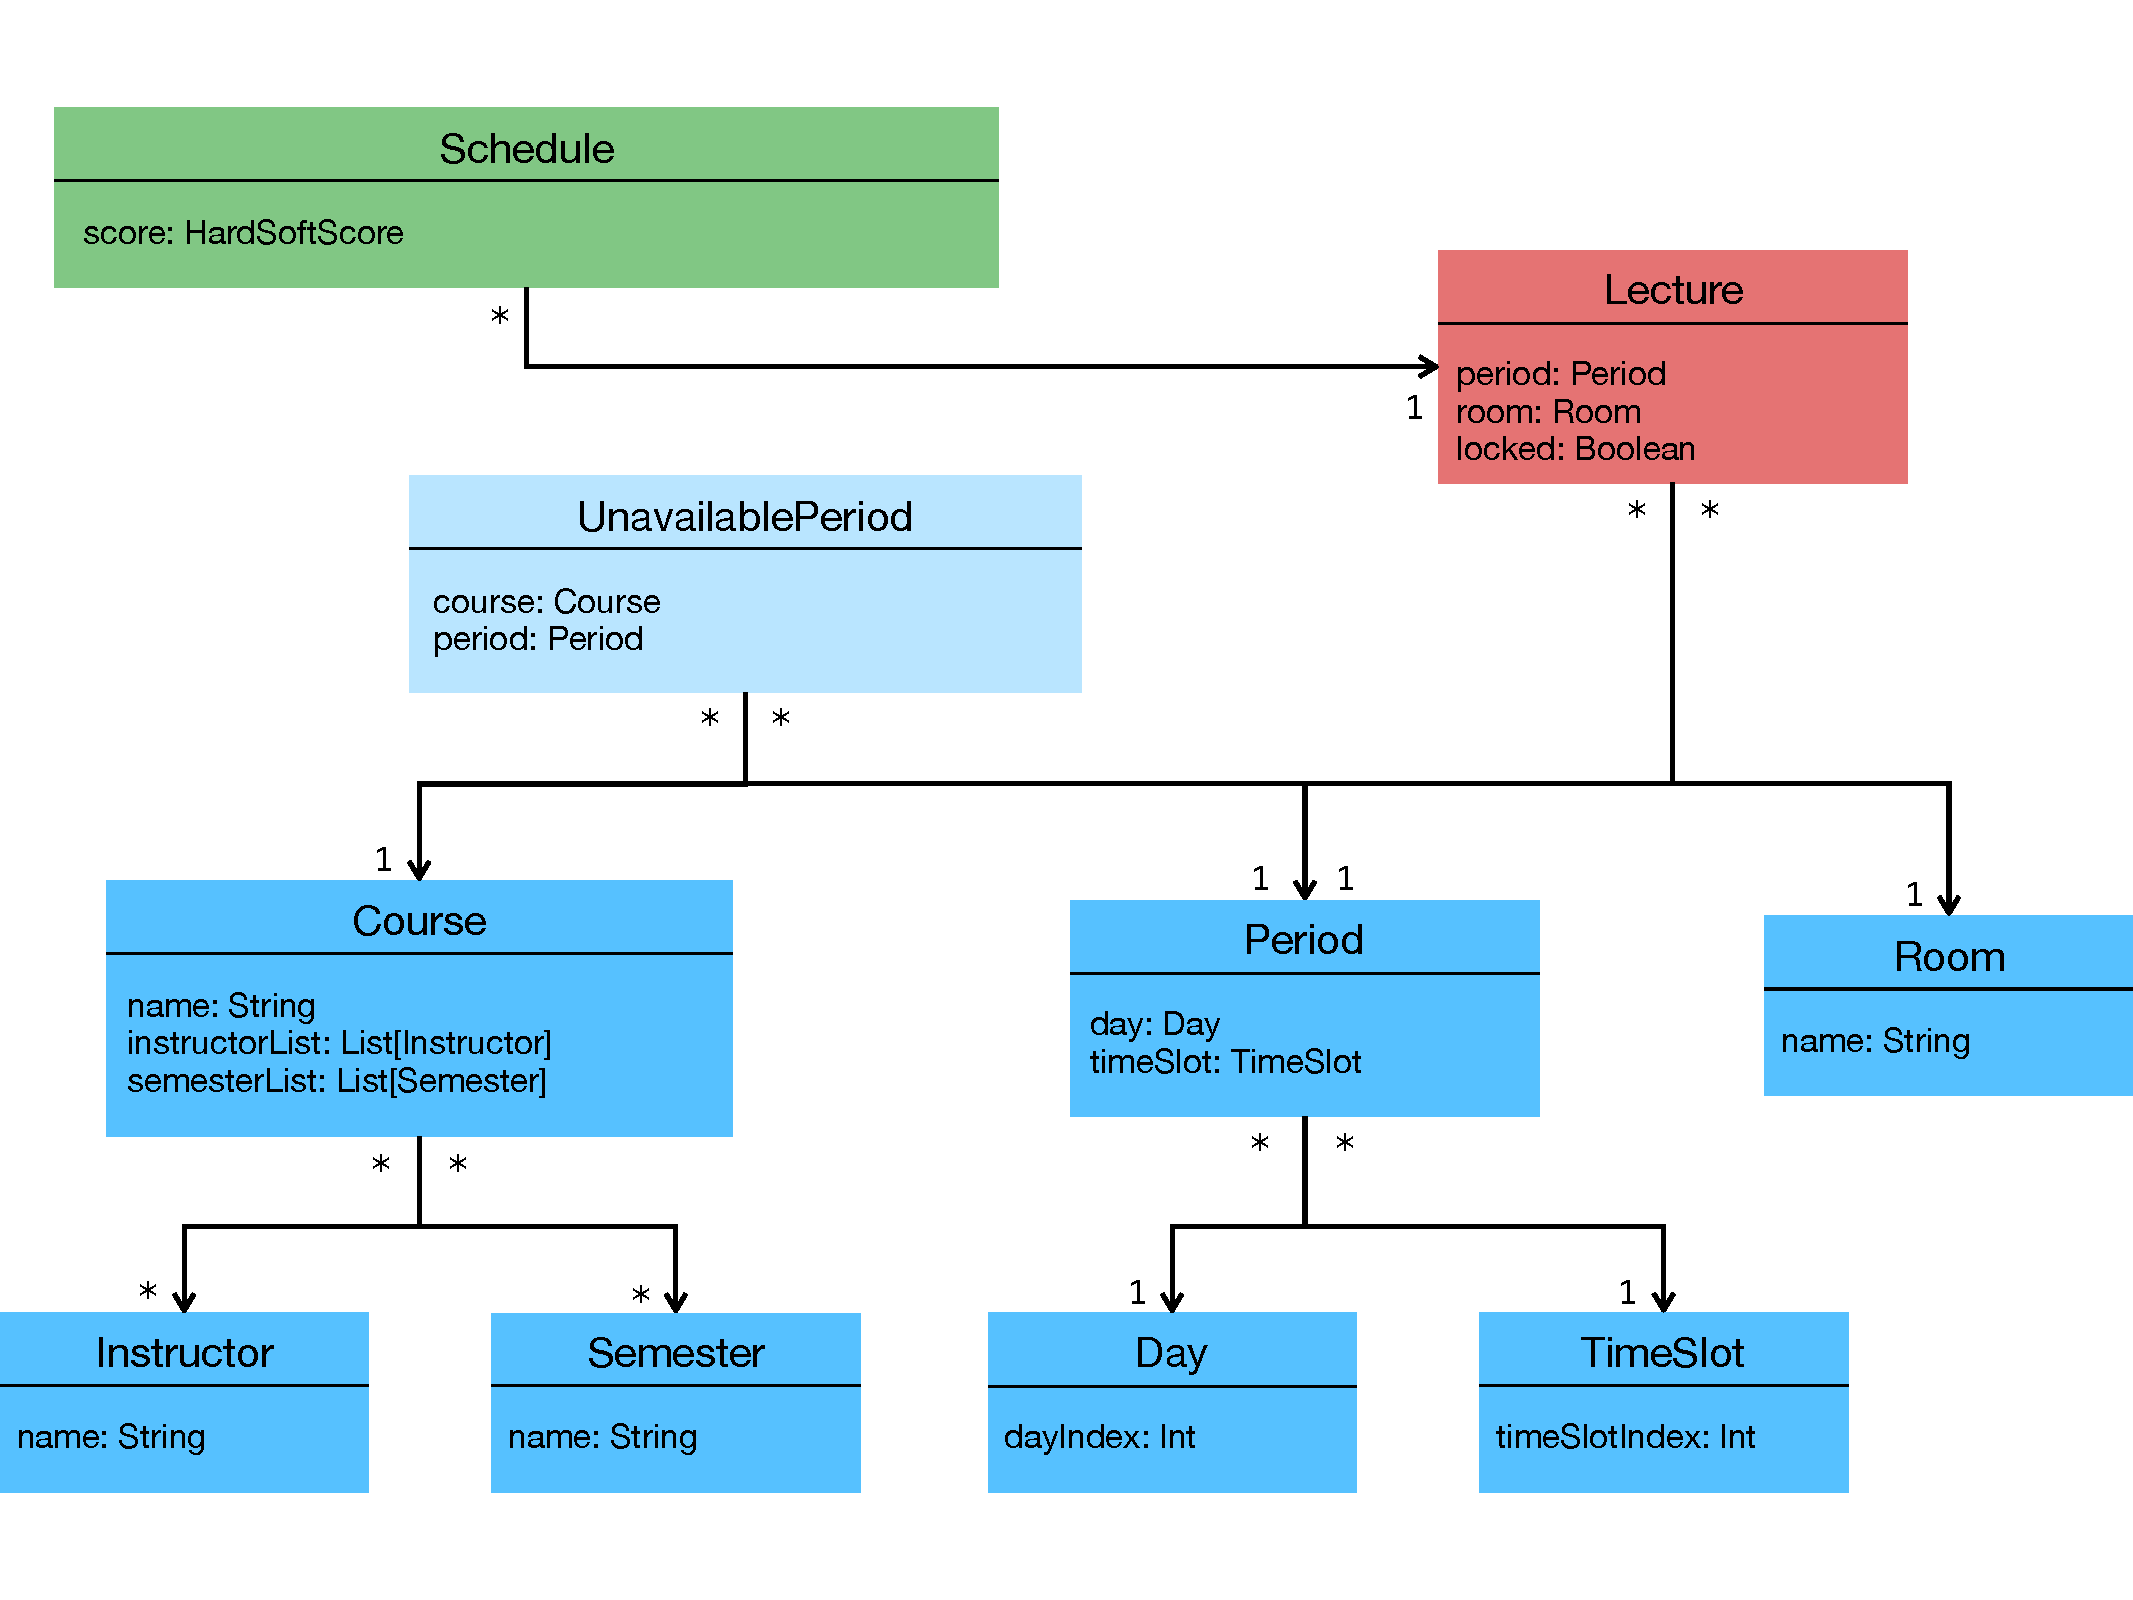
\includegraphics[width=\textwidth]{img/domainUML.pdf}
\caption{Class diagram of the domain model\label{fig:domainUML}}
\end{figure}
%To know more about the inner workings of OptaPlanner, see appendix \ref{appendix:optaplanner}.

%_______________________________________________________________________________
\section{Constraints\label{sec:constraints}}
The constraints are of two kinds, hard constraints and soft constraints, as described in Section \ref{sec:problem}.\par
As a rule, any solution that violates any hard constraint is unusable, since hard constraints model physical limitations (such as the impossibility for an instructor to teach two lectures at the same time).\par
To compute the score we need to take into account all constraint violations, so we need to iterate over all lectures and combine them with data from courses, rooms and unavailable periods.\par
A simple way to do this would be to accumulate constraint violations while iterating over all lectures combined with the other data. The problem with this approach is that the score needs to be calculated every time a new solution is created by the solver, i.e. many times per second, because the solver can mutate the solution very fast by just swapping two lectures or moving one single lecture.\par
It makes much more sense, from an efficiency point of view,  to remember which constraint violations did not change, and to just recompute the score with respect to the moved lecture (or swapped lectures).\par
To do this, we must rely heavily on maps, and the implementation can become very difficult to understand and to maintain.\par
Fortunately, OptaPlanner supports Drools, which is an engine that can automatically perform incremental score calculation given some rules. Each constraint is described as one or more rules. An example of a rule is available in Figure \ref{fig:rule}.\par
For most constraints it was possible to use the existing rules implemented in the OptaPlanner example, while for some others we had to apply some changes (we transformed the room capacity constraint into a hard constraint) or write the rule from the ground up (for the lecture pairs constraint; see Section \ref{sec:problem}).

\begin{figure}[h]
\centering
\begin{lstlisting}[language={[drl]Drools}]
// Room capacity: A room's capacity should not be
// less than the number of students in the course.
// Each student above the capacity counts as 1 point
// of penalty.
rule "roomCapacity"
	when
    	$room : Room($capacity : capacity)
	    Lecture(
			room == $room,
			course.studentSize > $capacity,
			$studentSize : course.studentSize
		)
	then
    	scoreHolder.addHardConstraintMatch(
			kcontext,
			($capacity - $studentSize)
		);
end
\end{lstlisting}
\caption{Rule that models the room capacity constraint\label{fig:rule}}
\end{figure}

%_______________________________________________________________________________
\section{Solver architecture\label{sec:solver}}
The solver (implemented in \cod{solver.SchedulerApp}) exposes a method \cod{solve(s: Schedule): Schedule} which expects a schedule with uninitialized lectures (no room or period assigned) or partially initialized lectures (if a lecture is locked, it \emph{must} have both a period and a room already assigned). Of course, the input data needs to be consistent: for example, no initialized lecture must be assigned to a room or a period that do not exist.\par
The solver is configured to run a construction heuristic phase which uses the First Fit Decreasing heuristic. The following two phases, which are local search phases, use Late Acceptance and Simulated Annealing.
The output is again a schedule, with all lectures assigned to a room and a period.\par
Both input and output objects of type \cod{Schedule} refer to the \cod{domain} implementation used by the solver, which uses simple syntax often similar to Java.

%_______________________________________________________________________________
\section{Server and GraphQL API\label{sec:graphql}}
As said, the solver lives on the back end, and it is available via a GraphQL endpoint. The server is implemented in Scala using Akka HTTP, and has one single endpoint: both \cod{/} and \cod{/graphql} are ways to access it.\par
The server stores (during runtime, there is no persistence) all courses, buildings, rooms, as well as a map that stores created schedules by ID. The ID of a Schedule is computed based on the courses and rooms chosen for scheduling.\par
All of this is stored as instances of Scala classes of the \cod{model} implementation, which are different from the classes used by the solver. The server in fact contains a class \cod{SchedulerRepo} which is responsible for the conversion between the two models when dealing with the solver.\par
The GraphQL interface provides queries and mutations, and they are listed in Table \ref{tab:graphql}.\par
\begin{table}[h]
\begin{tabularx}{\textwidth}{|l|X|}\hline
\multirow{2}{*}{\cod{query}} & \cod{buildings: [Building!]!} \\
& \cod{rooms: [Room!]!} \\
& \cod{courses: [Course!]!} \\
& \cod{semesters: [Semester!]!} \\
& \cod{plannerCourses: [Course!]!} \\
& \cod{plannerRooms: [Room!]!} \\
& \cod{plannerSchedule(id: Int!): Schedule} \\
& \cod{plannerSchedules: [Schedule!]!} \\\hline
\multirow{2}{*}{\cod{mutation}} & \cod{createSchedule(name: String!): Schedule} \\
& \cod{refineSchedule(id: Int!): Schedule} \\
& \cod{editLecture(id: Int!lectureArg: LectureInput!): Lecture} \\\hline
\end{tabularx}
\caption{GraphQL Schema exposed by the endpoint\label{tab:graphql}}
\end{table}
The table shows what is called a GraphQL Schema. Before the column we have the field name, after the column we have the field \cod{Type}. The exclamation mark means that the field is not nullable, and the square brackets indicate an array type.\par
For more information about GraphQL, see Appendix \ref{appendix:graphql}.

%_______________________________________________________________________________
\section{Web application UI\label{sec:polymer}}
We chose Polymer as a library to develop the front-end interface to use the solver.\par
The main page features two tabs: the first tab shows a list of buildings, and the plan was to show calendars with real events for every room once a building is opened. This idea was put aside to focus on implementing the functionalities of the second tab, which is the schedule creator.\par
The schedule creator shows a list of created schedules, starting with none. An ``add'' button on the bottom right can be used to open a page that shows the list of courses and rooms selected for scheduling. As of writing, it is not possible to change these selections, so it is possible to create just one of schedule, the one that uses the rooms and courses that are pre selected at server startup (for demonstrative purposes).\par
Creating a schedule is simple: it is sufficient to enter a name and click ``create''.\par
The home of the schedule creator can be seen in figure \ref{fig:creator}.

\begin{figure}[h]
\centering
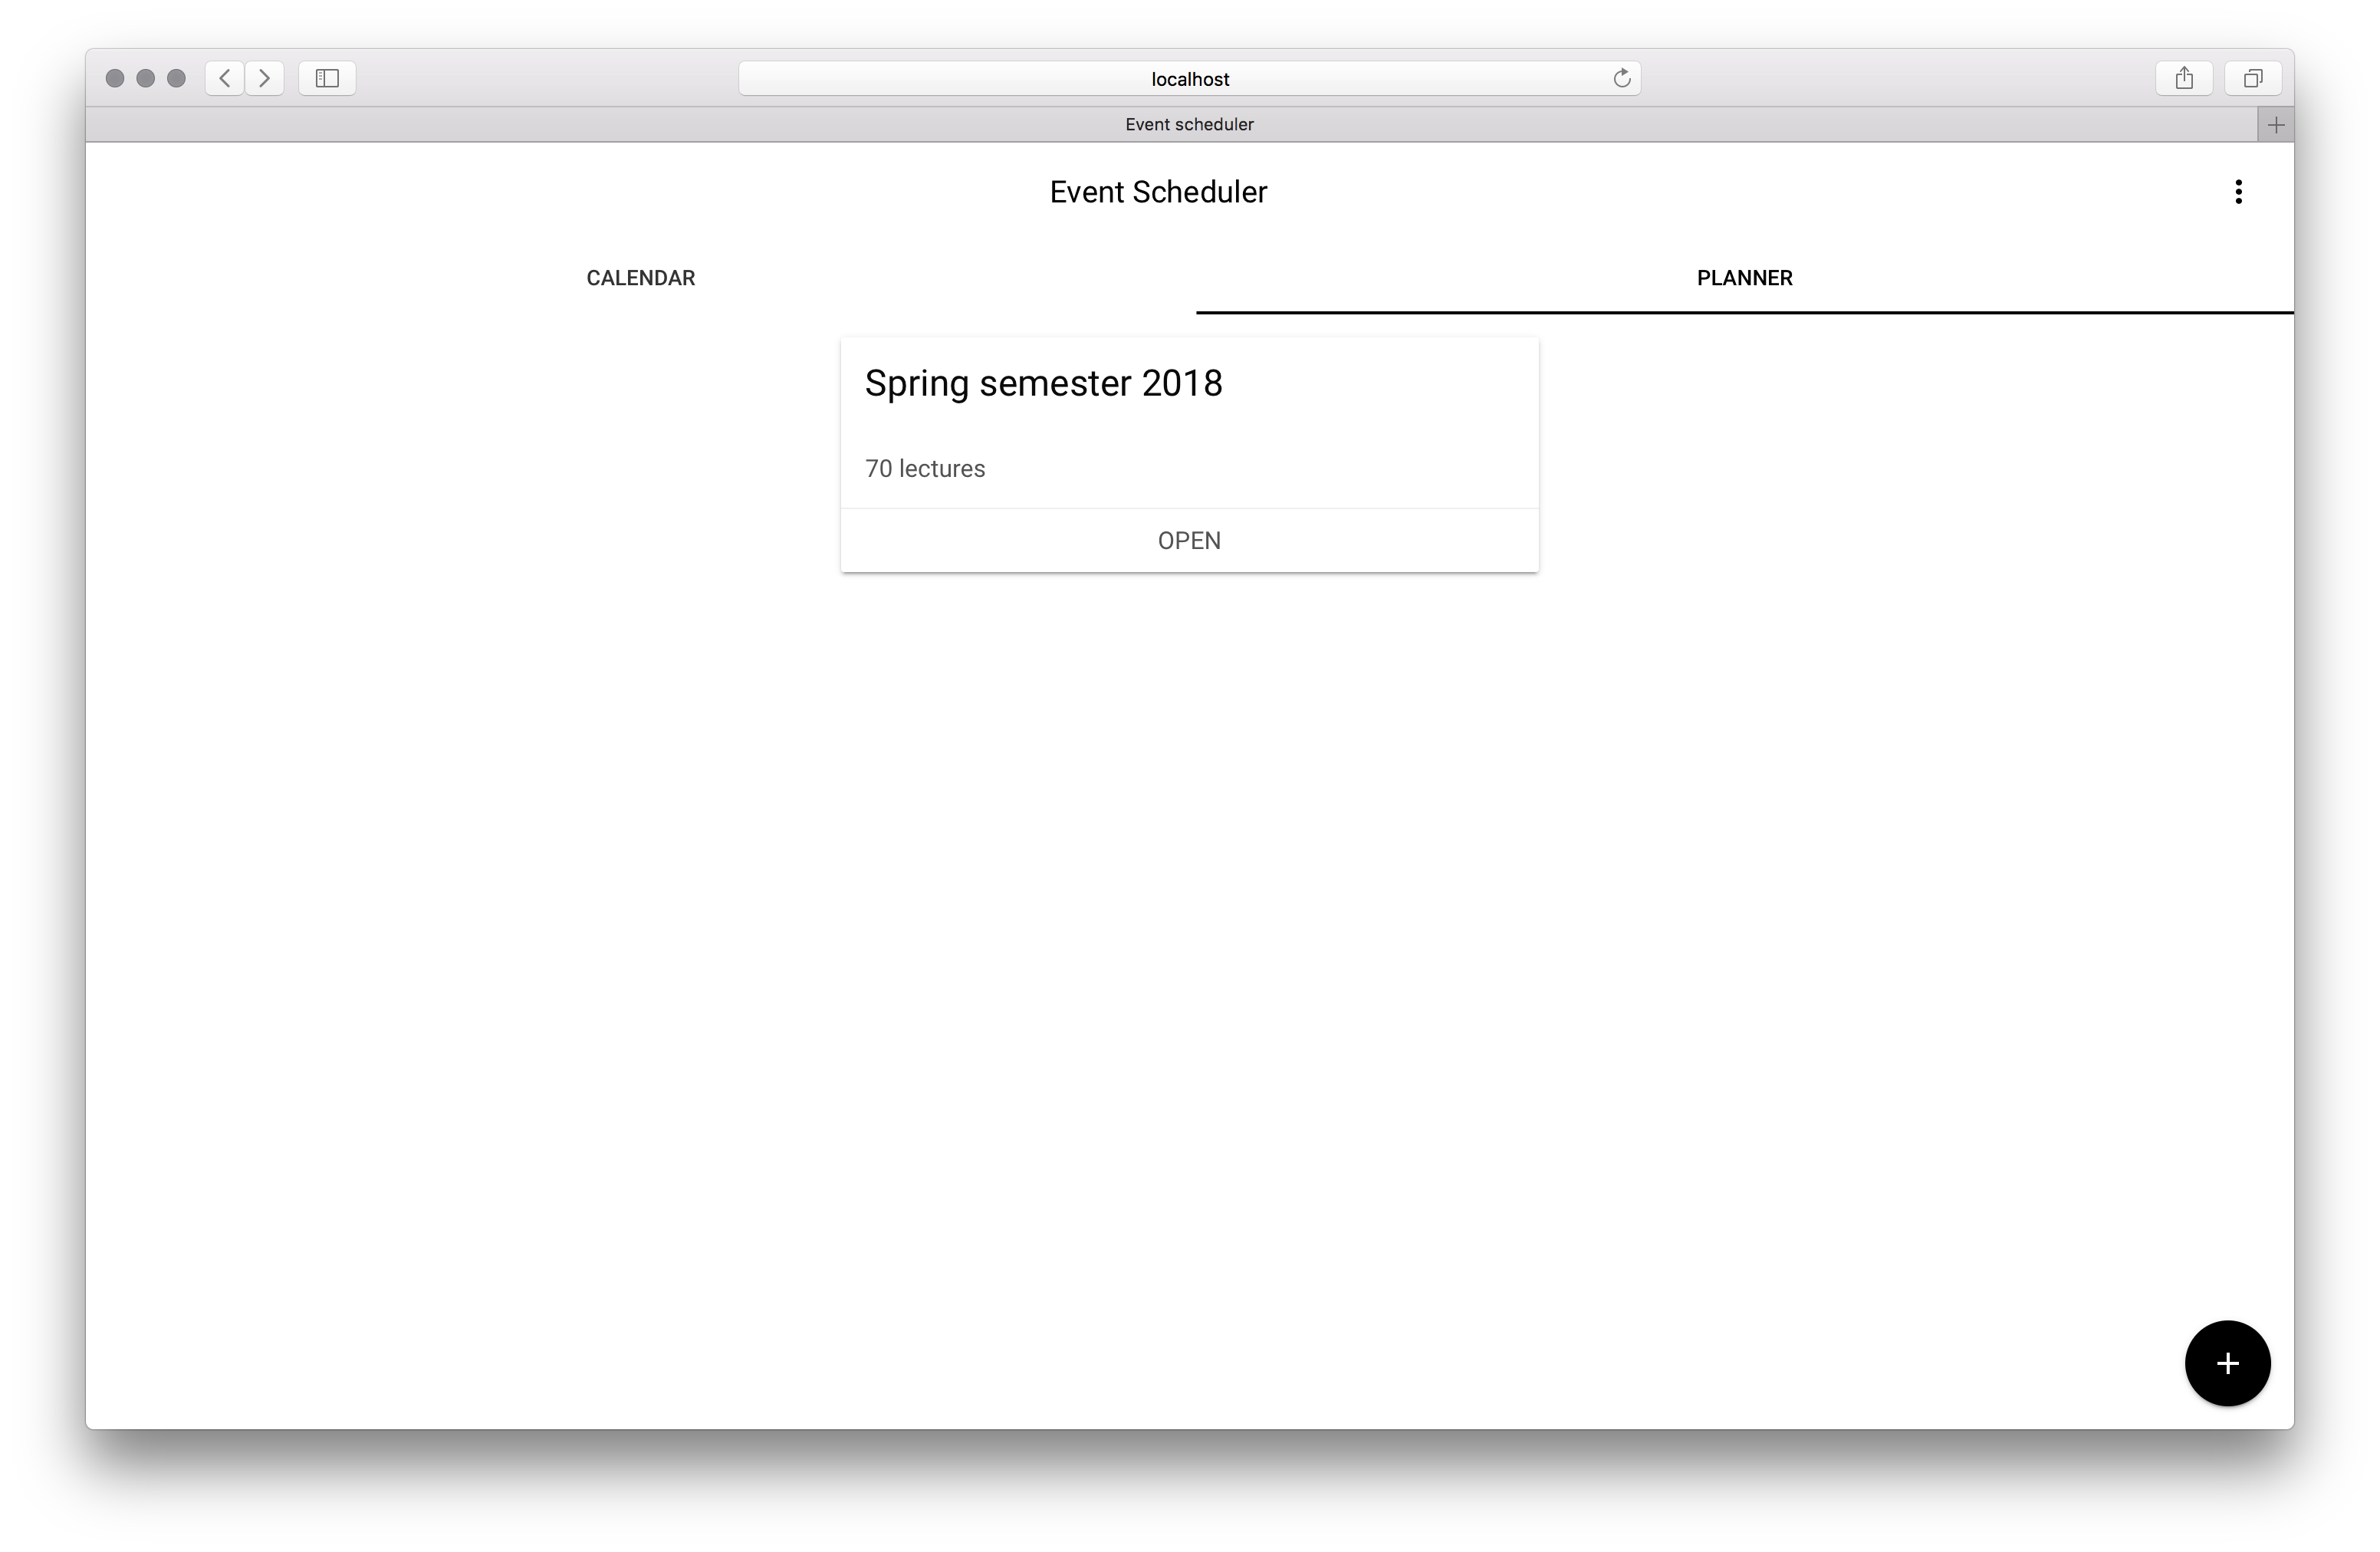
\includegraphics[width=\textwidth]{home.png}
\caption{Home of the planner \label{fig:creator}}
\end{figure}

By clicking on a schedule, a new view opens; on this view, the schedule is shown as a weekly timetable, separated by semester. If the schedule is the direct result of the solver, it is not possible to refine it, because the result would just be the same (see Figure \ref{fig:refined}). We call such a schedule ``refined''.\par

\begin{figure}[h]
\centering
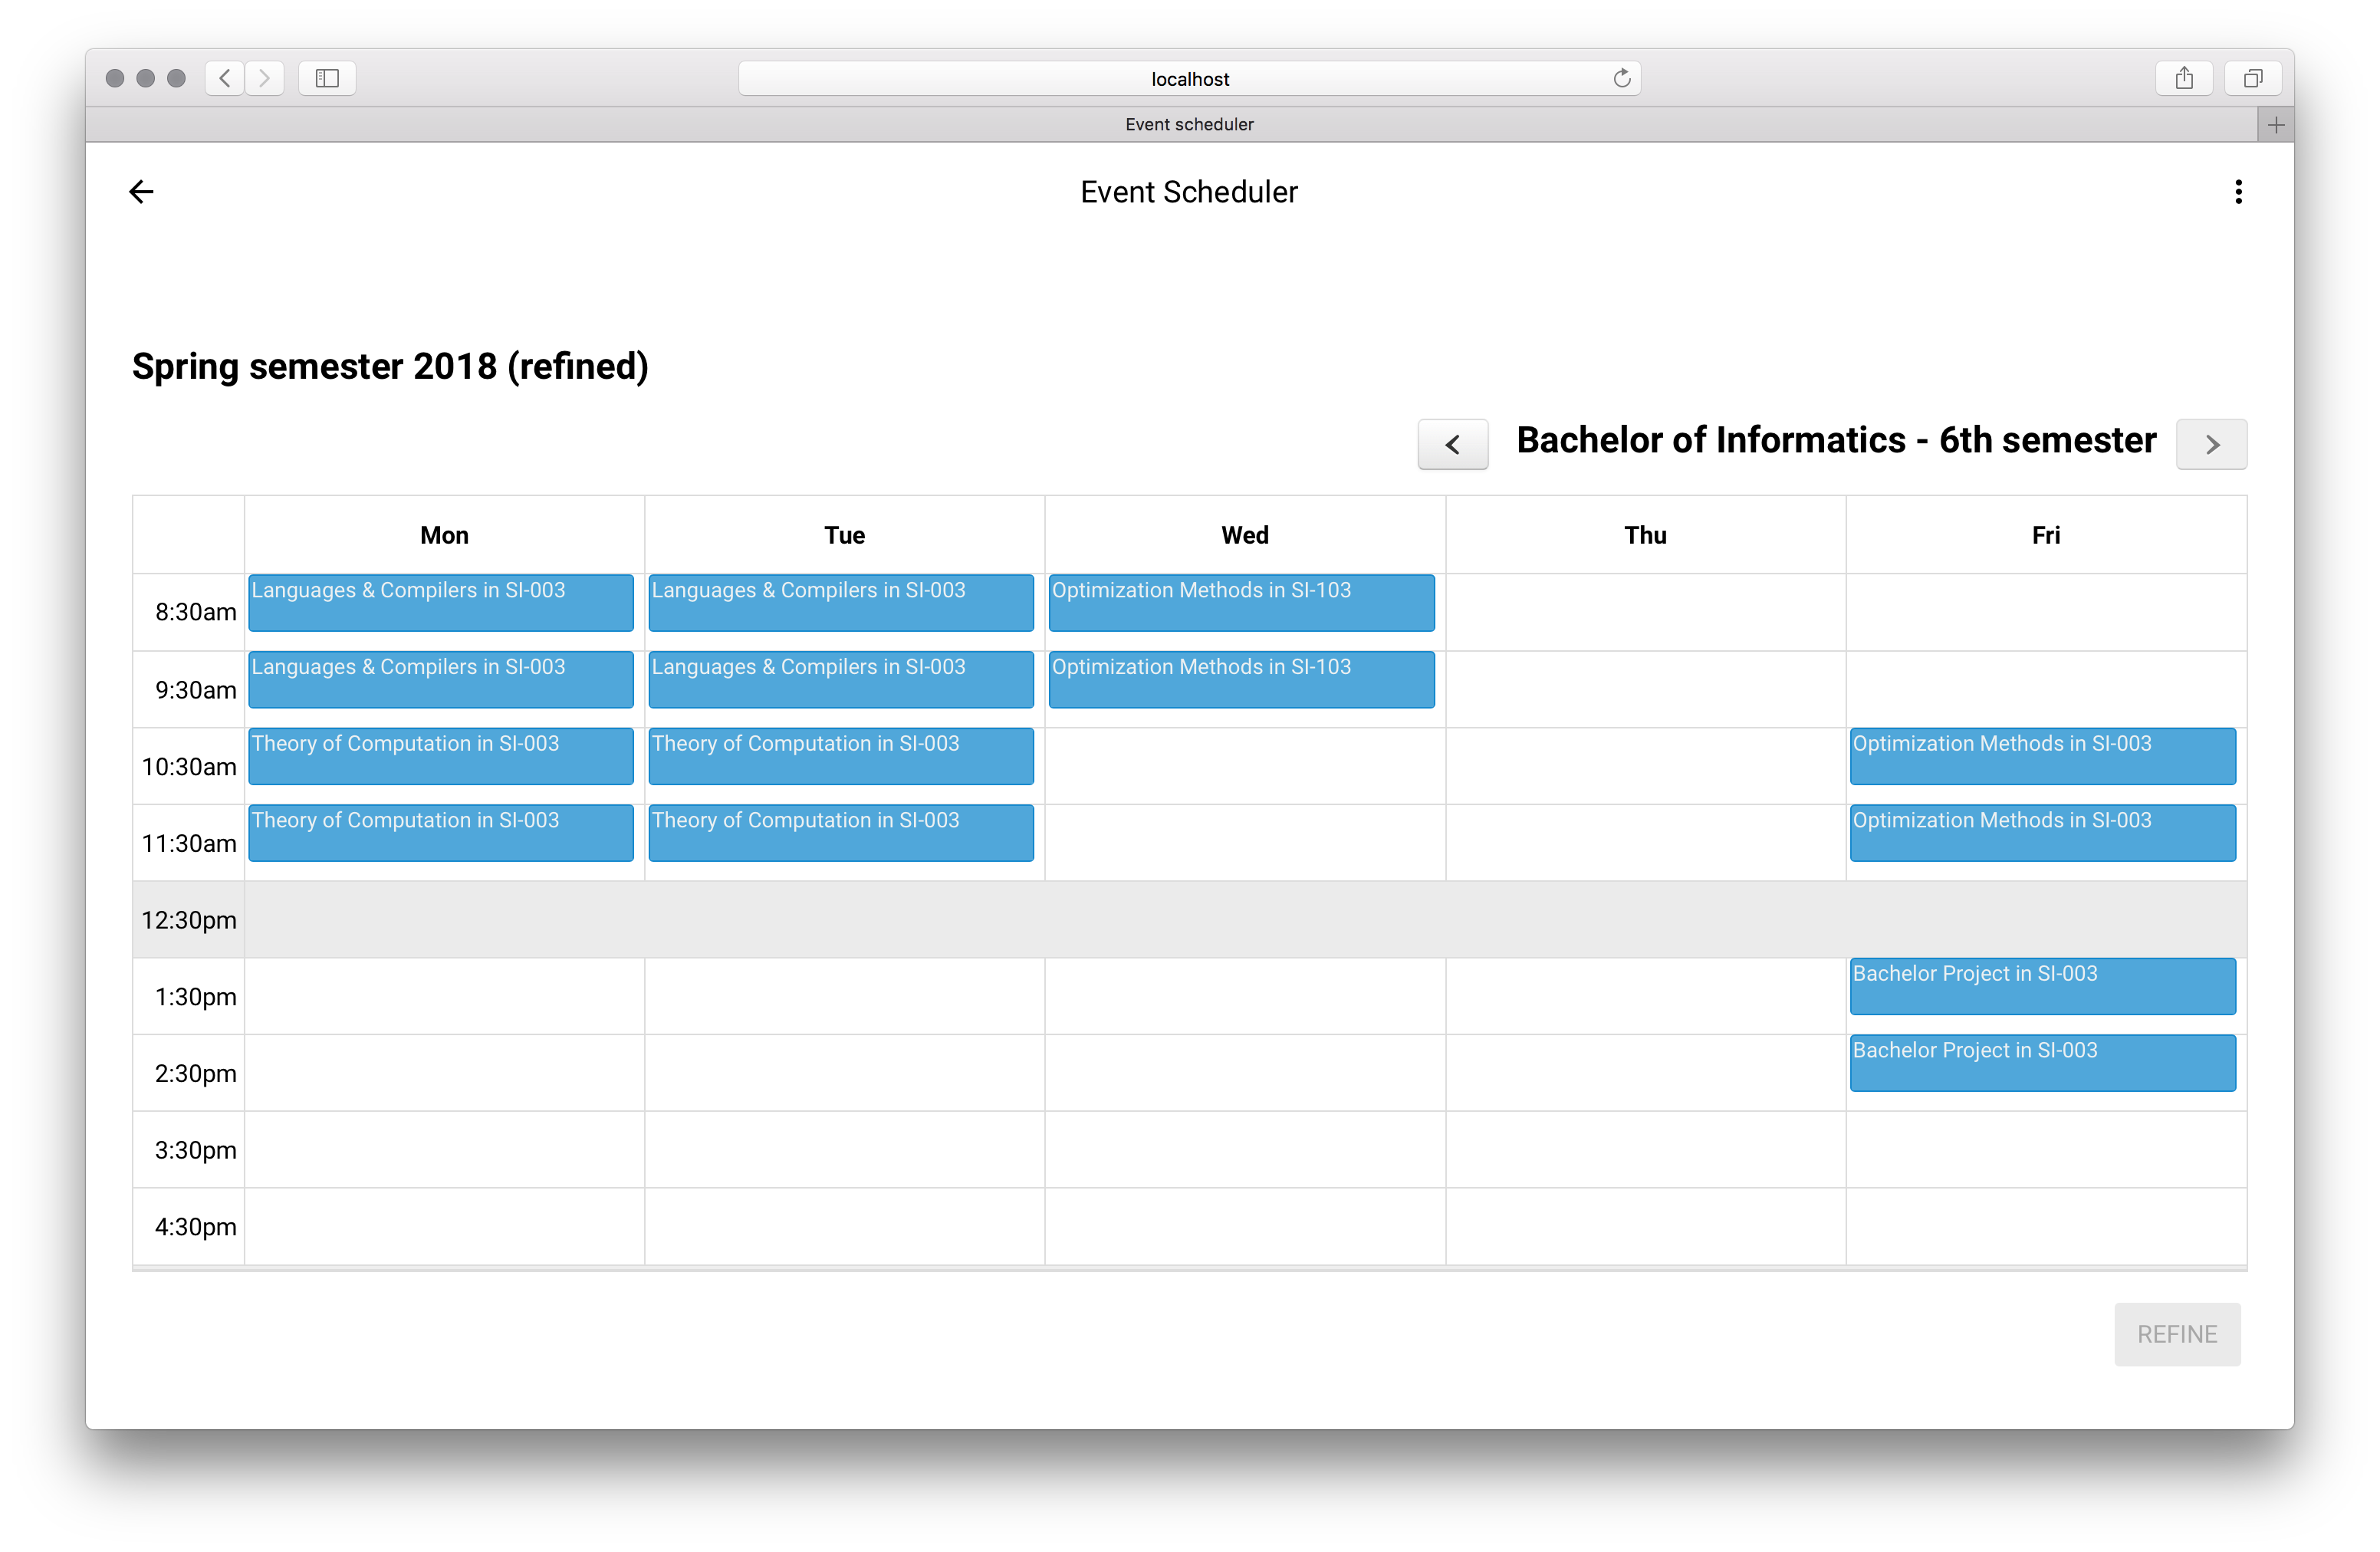
\includegraphics[width=\textwidth]{refined.png}
\caption{A refined schedule \label{fig:refined}}
\end{figure}

However, if it was modified, for example if a some lectures were moved and locked, it is possible to click the ``refine'' button (see Figure \ref{fig:notrefined}). This starts the solver on the back end using the already existing schedule; only locked lectures are preserved in place.\par

\begin{figure}[h]
\centering
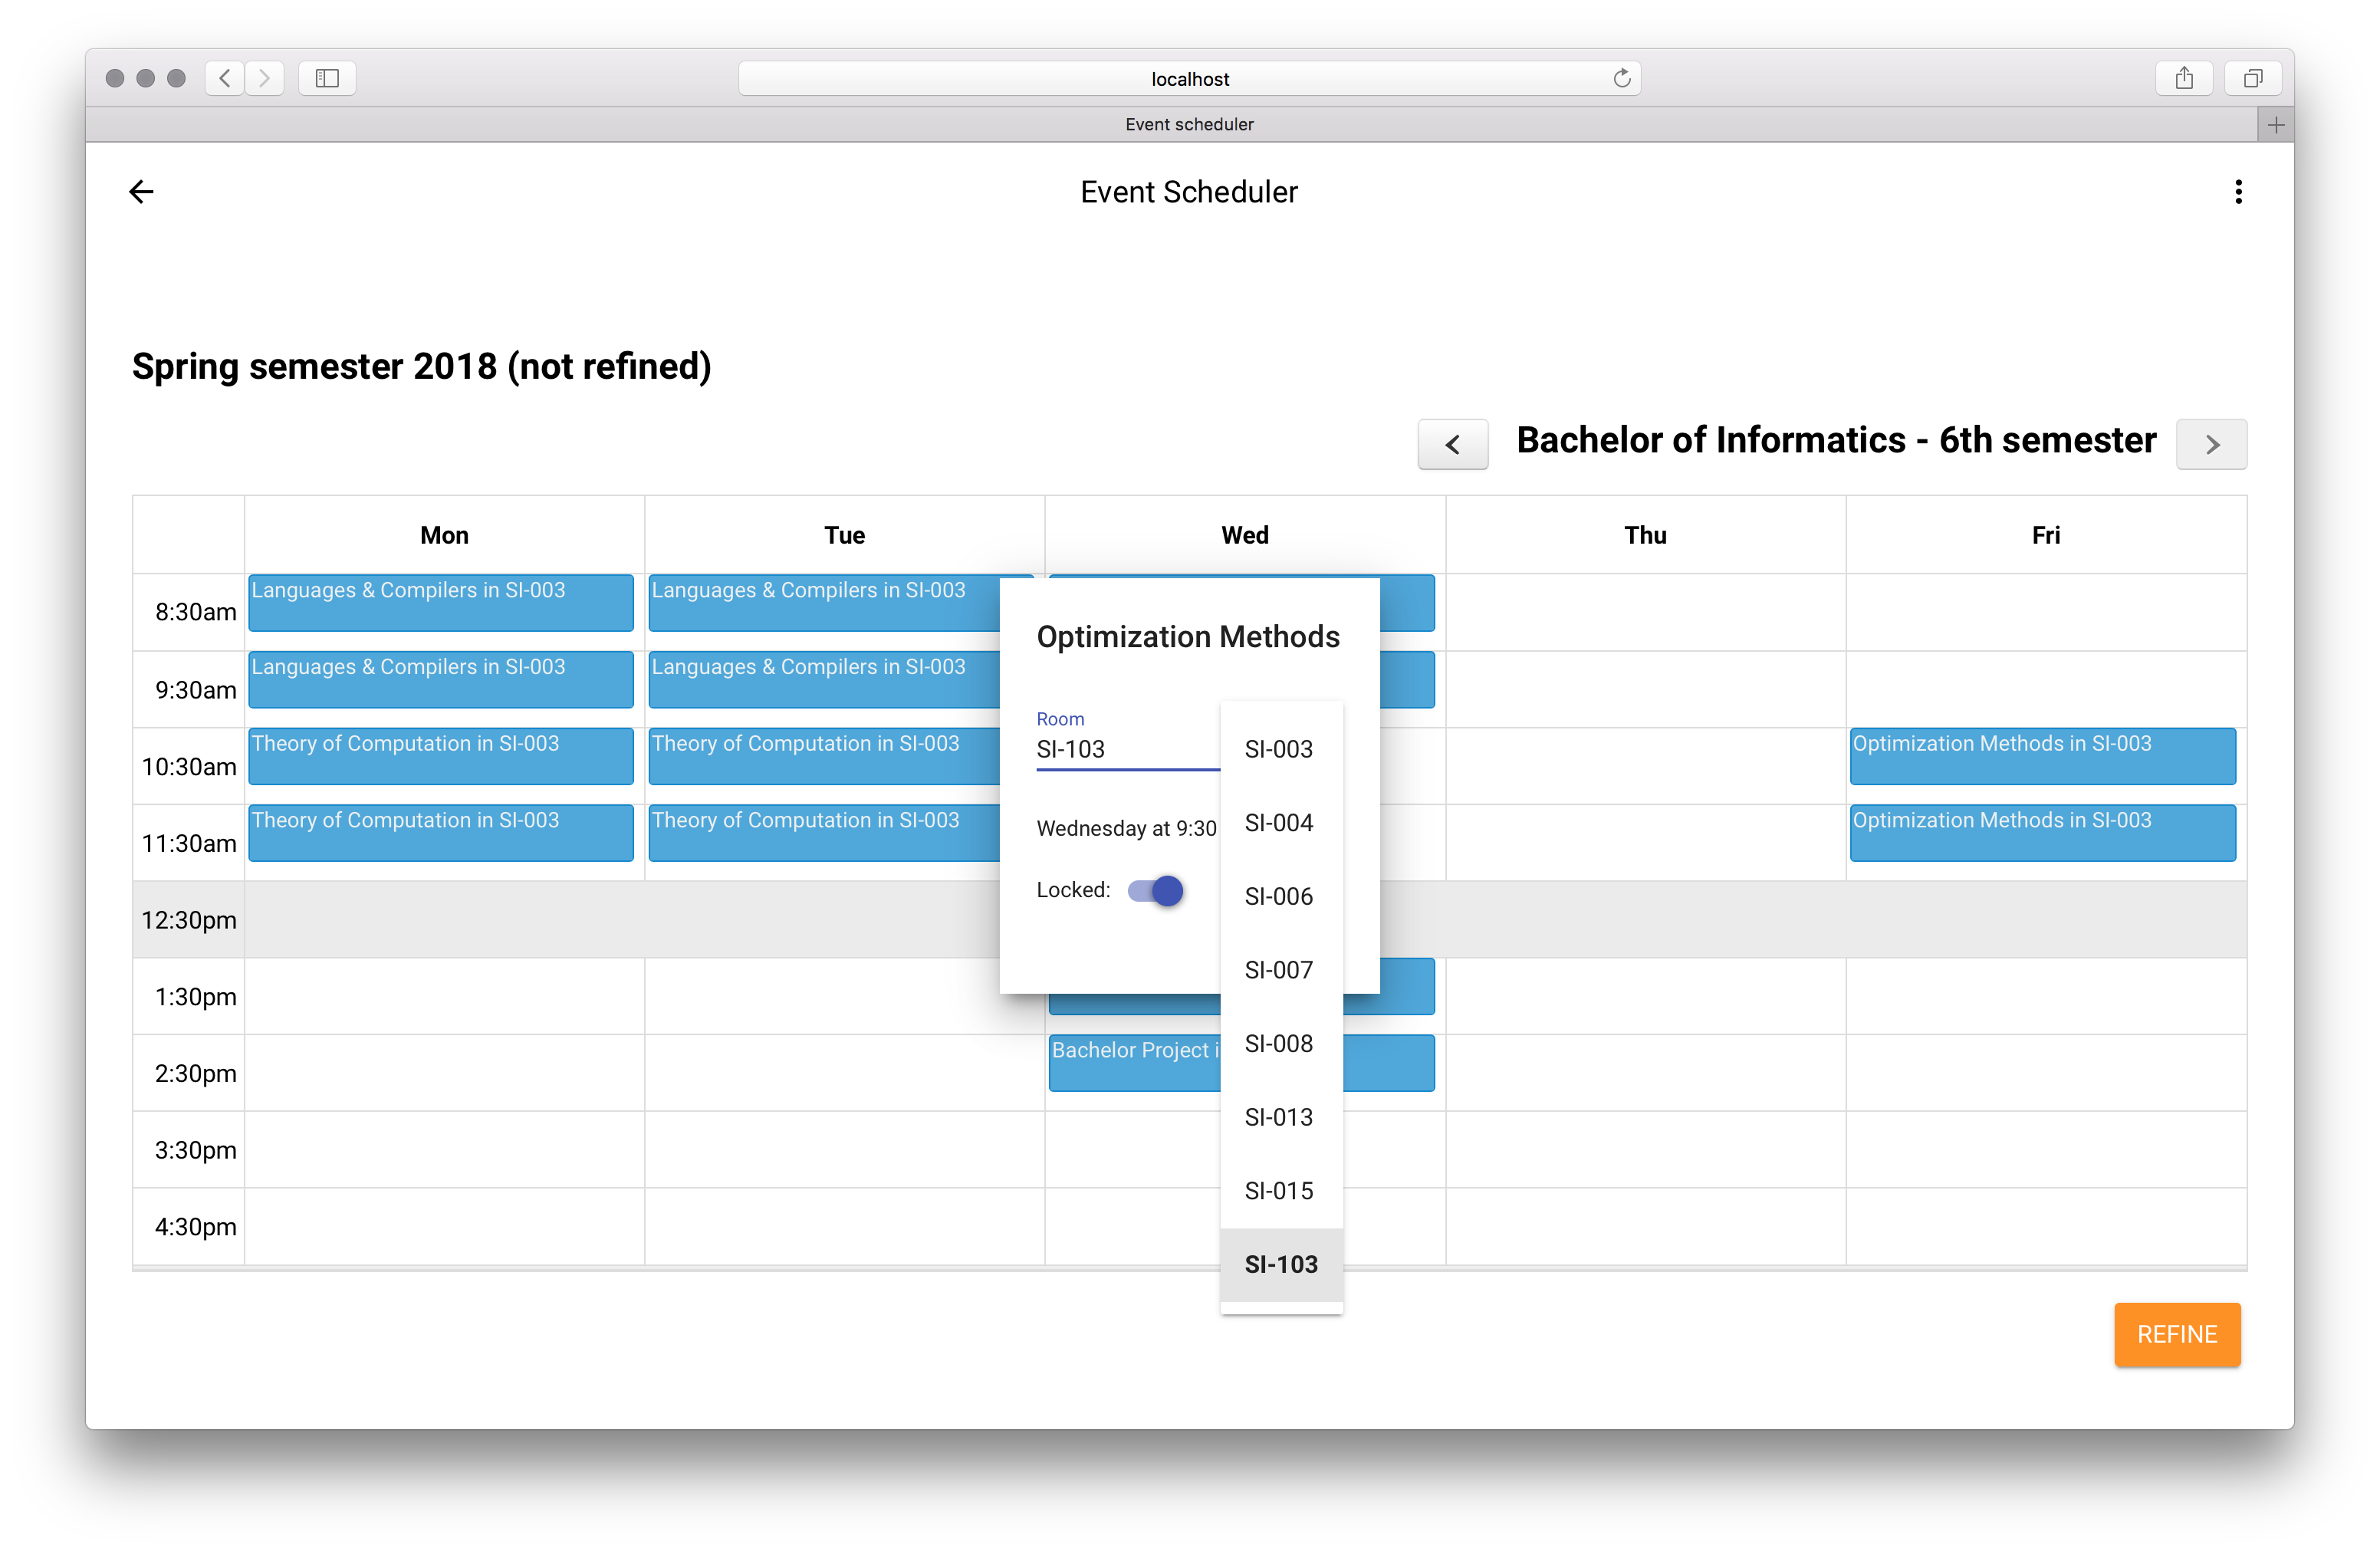
\includegraphics[width=\textwidth]{not_refined.png}
\caption{A non refined schedule \label{fig:notrefined}}
\end{figure}


%%%%%%%%%%%%%%%%%%%%%%%%%%%%%%%%%%%%%%%%%%%%%%%%%%%%%%%%%%%%%%%%%%%%%%%%%%%%%%%%
%%%%%%%%%%%%%%%%%%%%%%%%%%%%%%%%%%%%%%%%%%%%%%%%%%%%%%%%%%%%%%%%%%%%%%%%%%%%%%%%
\chapter{Conclusion}
The implemented solver produces good results which are comparable to those produced by the Dean's office, but in a much shorter time.\par
The application allows the user to create a schedule for a previously determined set of courses and rooms. The user can then visualize the solution, modify it and ask the solver to refine it. [...]

%_______________________________________________________________________________
\section{Evaluation}
During development, we tested the solver using as problem instance the data for the spring semester of the year 2018 of the Bachelor program of the Faculty of Informatics at USI\footnote{\url{http://www.inf.usi.ch}}. The problem instance features 3 semesters, with a total of 14 courses. The number of lectures is 70, and they need to be scheduled on a school week which counts 40 periods (8 time slots per day). As available rooms we used all the rooms of the Informatics Building, so 8 rooms.\par
The resulting schedules are produced in about 7 seconds, and are somewhat similar to the real timetables that are being used in the current semester. While the found solution does not violate any hard constraint, some soft constraints are violated, such as semester room stability and semester compactness (see Section \ref{sec:problem}).\par
Results are available in Appendix \ref{appendix:results}.

%_______________________________________________________________________________
\section{Future work}
The web application allows users to create a schedule for a given set of rooms and courses, with predefined unavailable periods. As a future work, the UI can be improved to enable the selection of specific courses, rooms, and other constraints.\par
Other possible extensions include approving a suitable schedule and publishing it to the official University calendar. This calendar may offer different ways to aggregate the events such as by room, instructor, user, or by day.\par
The calendar could also be augmented with the possibility to add non-recurring events such as seminars or conferences.

%%%%%%%%%%%%%%%%%%%%%%%%%%%%%%%%%%%%%%%%%%%%%%%%%%%%%%%%%%%%%%%%%%%%%%%%%%%%%%%%
%%%%%%%%%%%%%%%%%%%%%%%%%%%%%%%%%%%%%%%%%%%%%%%%%%%%%%%%%%%%%%%%%%%%%%%%%%%%%%%%
\appendix
%\chapter{OptaPlanner\label{appendix:optaplanner}}
%This is the OptaPlanner appendix...

\chapter{GraphQL\label{appendix:graphql}}
This appendix gives some examples of queries and responses using the schema defined in Section \ref{sec:graphql}.\par
To query for all buildings with their name and all the rooms inside them, each with name and capacity, we would use this query:
\begin{lstlisting}
query {
  buildings {
    name
    rooms {
      name
      capacity
    }
  }
}
\end{lstlisting}
The result of this query would be this (reduced):
\begin{lstlisting}[language=java]
{
  "data": {
    "buildings": [
      {
        "name": "Red Building",
        "rooms": [
          {
            "name": "A-11",
            "capacity": 165
          }, ...
        ]
      }, ...
    ]
  }
}
\end{lstlisting}



\chapter{Results\label{appendix:results}}
TODO: should the table go sideways and on a new page? Should I really show 6 tables (one per semester, both real and from solver)?\ppar
This appendix shows the results produced by the solver, followed by the real schedule that is being used in the spring semester of 2018 for the Bachelor of Informatics at USI.

%\begin{table}[h]
%\begin{tabularx}{\textwidth}{|r|X|X|X|X|X|}\hline\hline
%\textbf{Time} & \textbf{Mon} & \textbf{Tue} & \textbf{Wed} & \textbf{Thu} & \textbf{Fri} \\\hline\hline
%08:30 & L & L & L & L & L \\\hline
%09:30 & L & L & L & L & L \\\hline
%10:30 & L & L & L & L & L \\\hline
%11:30 & L & L & L & L & L \\\hline\hline
%13:30 & L & L & L & L & L \\\hline
%14:30 & L & L & L & L & L \\\hline
%15:30 & L & L & L & L & L \\\hline
%16:30 & L & L & L & L & L \\\hline
%\end{tabularx}
%\caption{Bachelor 2nd semester produced by the solver\label{tab:schedulerBSc2}}
%\end{table}

\begin{table}[h]
\begin{tabularx}{\textwidth}{|r|X|X|X|X|X|}\hline\hline
\textbf{Time} & \textbf{Mon} & \textbf{Tue} & \textbf{Wed} & \textbf{Thu} & \textbf{Fri} \\\hline\hline
08:30 & Programming Fundamentals 2 in SI-006 & L & L & L & L \\\hline
09:30 & L & L & L & L & L \\\hline
10:30 & L & L & L & L & L \\\hline
11:30 & L & L & L & L & L \\\hline\hline
13:30 & L & L & L & L & L \\\hline
14:30 & L & L & L & L & L \\\hline
15:30 & L & L & L & L & L \\\hline
16:30 & L & L & L & L & L \\\hline
\end{tabularx}
\caption{Bachelor 2nd semester produced by the solver\label{tab:schedulerBSc2}}
\end{table}

%%%%%%%%%%%%%%%%%%%%%%%%%%%%%%%%%%%%%%%%%%%%%%%%%%%%%%%%%%%%%%%%%%%%%%%%%%%%%%%%
%%%%%%%%%%%%%%%%%%%%%%%%%%%%%%%%%%%%%%%%%%%%%%%%%%%%%%%%%%%%%%%%%%%%%%%%%%%%%%%%
\bibliography{report}{}
\bibliographystyle{plain}

\end{document}
